\section{Cortex-M Architecture}

\section*{Registers}
\begin{itemize}
  \item 16 Core Registers
  \item 32-Bit wide
  \item RO-R7 Lower Registers
  \item R8 - R12 Higher Registers
  \item R13 Stack Pointer Temp Storage
  \item R14 Link Register Return from Procs
  \item R15 Program Counter Addr of next Instr.
\end{itemize}

\section*{ALU}
\begin{itemize}
  \item 32-Bit wide processing unit
\end{itemize}

\section*{APSR (Flag Register)}
\begin{itemize}
  \item N Negative
  \item Z Zero
  \item C Carry
  \item V Overflow
\end{itemize}

\section*{Instruction Set}
\begin{center}
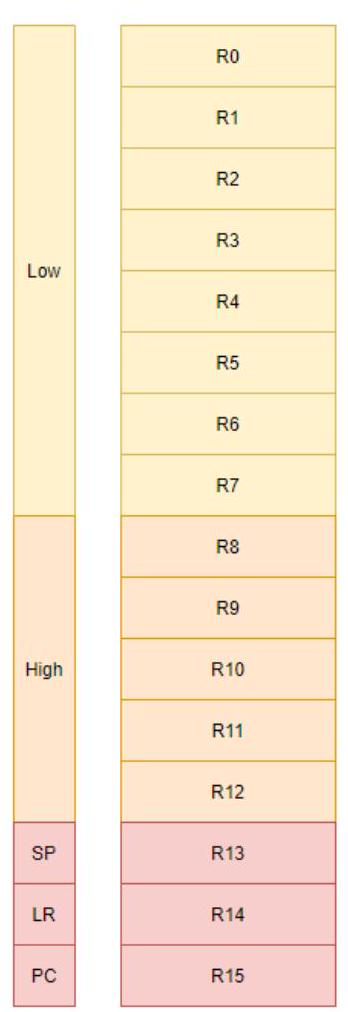
\includegraphics[width=\linewidth]{images/2024_12_29_79e6b22f503fb7b4f718g-02}
\end{center}

\begin{itemize}
  \item 16-Bit Thumb instruction encoding
\end{itemize}

\begin{center}
\begin{tabular}{llll}
Label & Instr. & Operands & Comments \\
\hline
demoprg & MOVS & R0,\#0xA5 & ; copy 0xA5 into register R0 \\
 & MOVS & R1,\#0x11 & ; copy 0x11 into register R1 \\
 & ADDS & R0,R0,R1 & ; add contents of RO and R1 \\
\end{tabular}
\end{center}

\section*{Instruction Types}
\begin{itemize}
  \item Data transfer
  \item Data processing
  \item Control flow Move, Load and Store\\
Arithmetic, Logical and Shift operations\\
Branches and functions
\end{itemize}

\section*{Assembly Program Structure}
\begin{center}
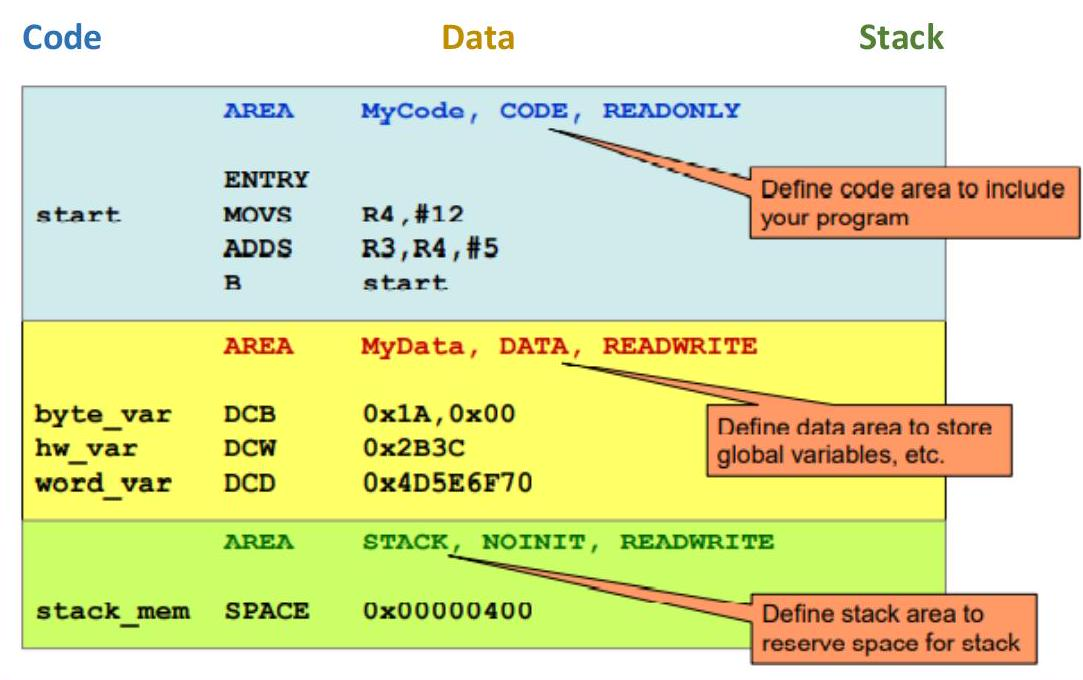
\includegraphics[width=\linewidth]{images/2024_12_29_79e6b22f503fb7b4f718g-02(1)}
\end{center}

Directives for initialized data

\begin{itemize}
  \item DCB Bytes
  \item DCW Half-Words
  \item DCD Words
\end{itemize}

\begin{center}
\begin{tabular}{|c|c|c|c|c|c|}
\hline
var1 & DCB & 0x1A &  &  &  \\
\hline
var2 & DCB & 0x2B & 0x3C & 0×4D & 0x5E \\
\hline
var3 & DCW & \multicolumn{2}{|r|}{0x6F70} & \multicolumn{2}{|c|}{0x8192} \\
\hline
var4 & $D C D$ & \multicolumn{4}{|c|}{0xA3B4C5D6} \\
\hline
\end{tabular}
\end{center}

Directives for uninitialized data

\begin{itemize}
  \item SPACE Bytes to be reserved
\end{itemize}